\subsection{Sebek}
Sebek ist ein Kernel basiertes Tool, welches die Daten eines Angreifers auf dem Host-System mitliest und loggt.\\ Zu beginn der Überwachung von Host-Systemen wurden häufig Netzwerk-Sniffer verwendet. Diese sind in der Lage alle Pakete zwischen Angreifer und Opfer-System mitzulesen. Damit sind Netzwerk-Sniffer in der Lage sowohl den Input als auch den Output zu rekonstruieren. In der heutigen Zeit wird es immer schwieriger an Daten wie beispielsweise Tastenanschläge zu kommen. Viele Hacker benutzen verschlüsselte Verbindungen zwischen ihren Opfer-Systemen und umgehen dadurch einem Netzwerk-Sniffer. Häufig wird für die Verschlüsselung SSH verwendet. Einige Angreifer verwenden eigene Tools, welche sie auf dem Opfer-System installieren um ihre Verbindung zu verschlüsseln. Um in solchen Fällen an die Daten des Angriffs zu kommen, mussten neue Methoden gefunden werden.

Aus dieser Not heraus entwickelte The Honeynet Project das Tool Sebek. Sebek konzentriert sich bei der Daten-Sammlung nicht auf die übertragenen Daten, sondern auf die Daten die im Kernel des Systems verarbeitet werden. Hintergrund dieses Vorgehens ist die Tatsache, dass verschlüsselte Daten nicht von dem System verarbeitet werden können. Somit kommen die Daten im Kernel unverschlüsselt zur Verarbeitung an. Durch dieses Vorgehen ist es für Sebek unerheblich welche Verschlüsselung von den Angreifern eingesetzt wird, da die Angreifer auch die Entschlüsselung für Sebek übernehmen. Sobald die Daten an dem System-Aufruf read() ankommen greift Sebek die Daten ab ohne dabei Aufsehen zu erregen.  

\begin{figure}[ht]
    \centering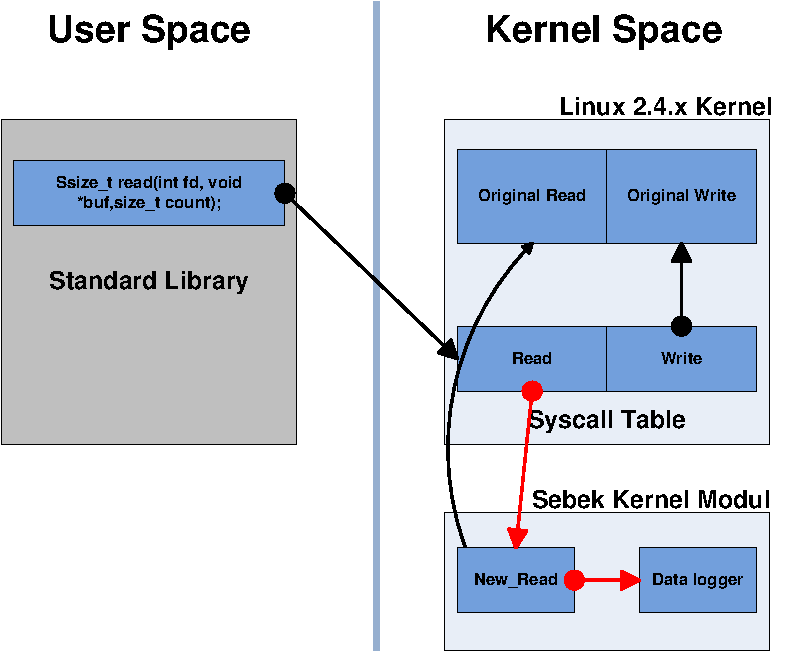
\includegraphics[scale=0.70]{Bilder/Sebek.pdf}
  \caption{Abfangen der Daten durch Sebek\cite{project.2003b}}
  \label{hnet:sebek}
\end{figure}

Möglich macht dieses Vorgehen die Manipulation des System-Aufrufs. Durch Sebek wird der Pointer, welcher in der Syscall Tabelle gespeichert wird, auf die read() Methode geändert. Der kompromittierte Pointer verweist nun auf eine von Sebek initialisierte read() Methode. Diese schreibt alle Informationen in einen \grqq Data logger\grqq und ruft danach die Originale read() Methode auf. Somit bekommt der Angreifer nicht mit, dass die Daten über einen Umweg abgefangen werden konnten. Um den Vorgang zu verdeutlichen wird dieser in Abb. \ref{hnet:sebek} bildlich dargestellt.

Ein weiteres Problem was nun entsteht, ist die Frage was mit den gesammelten Daten passiert. Um weiterhin im verborgenen zu bleiben, können die Daten nicht auf dem Host gespeichert werden. Hier hätte der Angreifer die Möglichkeit nach auffälligen Dateien zu suchen oder auch durch Zufall darauf zu stoßen. Dieses Problem umgeht Sebek indem die Daten kurz in dem Data logger gespeichert werden und von dort an einen Server geschickt werden. Diese Übertragung muss jedoch so vollzogen werden, dass der Angreifer keine Möglichkeit hat sie zu entdecken.
\begin{figure}[ht]
    \centering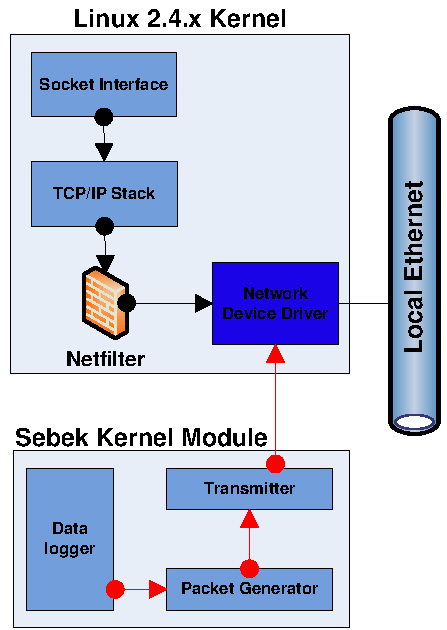
\includegraphics[scale=0.70]{Bilder/sebek_Network_Driver.pdf}
  \caption{Zugriff auf Netzwerk Driver\cite{project.2003b}}
  \label{hnet:sebekDriver}
\end{figure}
Um unerkannt zu bleiben werden die Pakete nicht über den TCP/IP Stack in das Netzwerk geleitet, sondern, wie ich Abb. \ref{hnet:sebekDriver} veranschaulicht, über den direkten Weg an den Netzwerk-Driver gesendet. Dadurch kann das System die Pakete weder durch einen Sniffer erkennen, noch über IPTABLES blockieren.
Der Angreifer hat nun noch die Möglichkeit über das mitlesen des LAN-Traffics Sebek-Pakete zu entdecken. Sollten sich mehrere Honeypots im Netzwerk befinden, können auch Sebek-Pakete von anderen Systemen mitgelesen werden. Dies gilt es zu verhindern um keinen Verdacht zu erwecken. Um die Pakete nicht entdecken zu können, implementiert Sebek eine eigene Version des Raw Socket Interface. Das Interface erkennt anhand des Ziel UDP-Ports und einem \grqq Magic-Value\grqq, welcher im Header der Pakete steht, dass es sich um ein Sebek-Paket handelt. Das Raw Socket Interface wird von Sebek so verändert, dass alle Sebek-Pakete verworfen werden und damit für jeden Sniffer auf einem Honeypot-Systeme unerkannt bleiben. Mit diesem Vorgehen schafft Sebek eine lückenlose Überwachung ohne dabei entdeckt zu werden. Ein beispielhafter Aufbau eines Angriffs-Szenario ist in Abb. \ref{hnet:sebekAufbau} dargestellt.\cite{project.2003b}
\begin{figure}[ht]
    \centering\includegraphics[scale=0.70]{Bilder/sebek_Aufbau.pdf}
  \caption{Ablauf einer Sebek-Überwachung\cite{project.2003b}}
  \label{hnet:sebekAufbau}
\end{figure}
